
\chapter*{The Wave Equation: Steady State and Resonance}
\addcontentsline{toc}{chapter}{The Wave Equation: Steady State and Resonance} 
\section*{Python Mechanics}
\addcontentsline{toc}{section}{Python Mechanics} 

\paragraph*{P3.1} Work through Chapter 3 of Introduction to Python, where you will learn
about user-defined functions and good commenting practices. For the
remainder of the course, you will need to demonstrate good commenting
practices in your code before your exercises will be passed off.
\section*{Wave Equation}
\addcontentsline{toc}{section}{Wave Equation} 

We are now ready to tackle our first partial differential equation: the wave equation. For a string of length L fixed at both ends with a force applied to it that varies
sinusoidally in time, the wave equation can be written as


\begin{equation}\label{eq:31}
		\mu \frac{\partial^2 y}{\partial t^2} = T \frac{\partial^2y}{\partial x^2} + f(x) \cos \omega t ; y(0,t) = 0, y(L,t) = 0
				\end{equation}
				
		where $y(x,t)$ is the lateral displacement of the string as a function of position
and time, assuming that $y(x,t) ≪ L.$
1 We have written Eq. \eqref{eq:31} in the form of
Newton\rq s second law, $F = ma$. The “ma” part is on the left of the equation, except
that $\mu$ is not the mass, but rather the linear mass density (mass per length). This
means that the right side should have units of force/length, and it does because
T is the tension (force) in the string and $\partial^2y / \partial x^2$
 has units of 1/length. Finally,
$f (x)$ is the amplitude of the driving force (in units of force/length) applied to the
string as a function of position (so we are not necessarily just wiggling the end of
the string) and ω is the frequency of the driving force. \\
Before calculating, let\rq s train our intuition to guess how the solutions of this
equation behave. If we suddenly started to push and pull on a string under tension
with force density $f(x)\cos(\omega t)$, we would launch traveling waves, which would
reflect back and forth on the string as the driving force continued to launch more
waves. The string motion would rapidly become very messy. But suppose that
there is a bit of damping in the system (not included in the equation above, but in
Lab 5 we will add it). With damping, all of the transient waves due to the initial
launch and subsequent reflections would die away and we would be left with a
steady-state oscillation of the string at the driving frequency $\omega$. This behavior is
the wave equation analog of damped transients and the steady final state of a
driven harmonic oscillator which you studied in Physics 330.		

\section*{Steady state solution by separation of variables}
\addcontentsline{toc}{section}{Steady state solution by separation of variables} 
Let\rq s look for this steady-state solution by guessing that the solution has the form
\begin{equation}\label{eq:32}
		y(x,t) = g(x)\cos(\omega t)
				\end{equation}
				This function has the form of a spatially dependent amplitude $g (x)$ which oscillates in time at the frequency of the driving force. Substituting this \lq\lq guess \rq\rq into the
wave equation and carrying out the derivatives yields (after some rearrangement)
\begin{equation}\label{eq:33}
		Tg^{\prime\prime}(x) + \mu \omega ^ 2 g(x) = -f(x) ; g(0) = 0, g(L) = 0
				\end{equation}
				This is just a two-point boundary value problem of the kind we studied in Lab 2,
so we can solve it using our matrix technique.
\paragraph*{P3.2}
	\marginpar{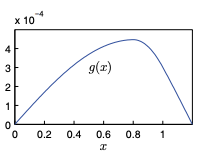
\includegraphics[width=\marginparwidth]{fig31}\captionof{figure}{Solution to P3.2(a)}\label{fig:15}}
\begin{enumerate}[label=(\alph*)]
	\item Write a program to solve Eq. \eqref{eq:33} for $N = 100$ points with $ \mu = 0.003,
T = 127, L = 1.2$, and $\omega = 400$. All quantities are in SI units. Find the
steady-state amplitude associated with the driving force density:
\begin{equation}\label{eq:34}
		f(x) = 
		\begin{cases}
		0.73 \ if \ 0.8 \	\geq x 	\geq 1 \\
		0 \ \ otherwise
		\end{cases}
				\end{equation}which is something like grabbing the string toward one end and wiggling. Plot $g(x)$, and properly label the axes of your plot.
				\item Take your code from (a) and turn it into a library with two functions:
				\begin{enumerate}
				\item	A function force that accepts the grid $x$ as an argument and
returns the column vector representing $f(x)$

\item A function $steadySol$ that accepts the arguments $f(x)$ (returned
from force), $h$, $\omega$, $T$ , and $\mu$. This function should construct the
matrix, solve the matrix equation, and return $g(x)$.
\end{enumerate}

	\marginpar{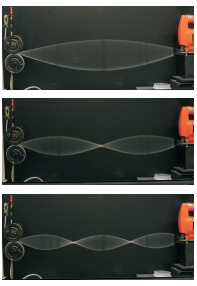
\includegraphics[width=\marginparwidth]{fig32}\captionof{figure}{Photographs of the first three resonant modes for a string fixed at both ends.}\label{fig:16}}
Save this library as “Lab3Funcs.py” and then write another program
that imports this library. In this program, write a $for$ loop that sweeps
the value of $\omega$ from $\omega = 400$to $\omega = 1700$ in 200 steps keeping the
values of the other parameters constant. Plot $g(x)$ at each frequency
so that you make an animation of what happens when you sweep the
driving frequency. Here is some example code to help you make the
animation, assuming you\rq ve stored your ω values in wplot:
		\begin{lstlisting}
		plt.figure(1)
for n in range(len(wplot)):
w = wplot[n]
g = l3.steadySol(f,h,w,T,u)
plt.clf() # Clear the previous plot
plt.plot(x,g)
plt.title('$\omega={:1.2e}$'.format(w))
plt.xlabel('x')
plt.ylim([-0.05, 0.05]) # prevent auto-scaling
plt.draw() # Request to draw the plot
plt.pause(0.1) # Allow time to draw it
		
\end{lstlisting}
	\marginpar{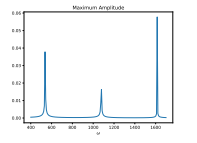
\includegraphics[width=\marginparwidth]{fig33}\captionof{figure}{Solution to problem 3.2(c).}\label{fig:16}}
At certain frequencies, you should see distinct resonance modes appear as in Fig. 3.2.
\item Modify your code from part (b) so that you find and record the maximum amplitude of $g(x)$ at each $\omega$. Then plot the maximum amplitude
as a function of ω to see the resonance behavior of this system. Describe what the peaks in this plot mean.
				
				
\end{enumerate}
				The height of the peaks in this Fig. 3.3 isn\rq t meaningful—the height of the
actual peak is essentially infinite (since we don’t have any damping yet), while
the height displayed on the plot is just a reflection of how closely our chosen
frequencies happened to line up with the exact resonance frequency. Now we will
learn how to find these resonant frequencies directly without needing to solve
the differential equation over and over again.

\section*{Resonance and the eigenvalue problem}
\addcontentsline{toc}{section}{Resonance and the eigenvalue problem} 
The essence of resonance is that at certain frequencies a large steady-state amplitude is obtained with a very small driving force. To find these resonant frequencies
we seek solutions of Eq. \eqref{eq:33} for which the driving force is zero. With $f(x) = 0$,
Eq. \eqref{eq:33} takes on the form

\begin{equation}\label{eq:35}
		Tg^{\prime\prime}(x) + \mu \omega ^ 2 g(x) = 0 \ ; \ g(0) = 0, g(L) = 0
				\end{equation}
				If we rewrite this equation in the form
				\begin{equation}\label{eq:36}
		g^{\prime\prime}(x) = - (\frac{\mu \omega^2}{T}g(x)
				\end{equation}
				
				\begin{equation}\label{eq:37}
		Ag =\lambda g
				\end{equation}
				where A is a linear operator (the second derivative on the left side of Eq. \eqref{eq:36} )
and $\lambda$ is the eigenvalue $(−\mu \omega^2 / T )$.
Equation \eqref{eq:36} is easily solved analytically, and its solutions are just the familiar
sine and cosine functions. The boundary condition $g (0) = 0$ tells us to try a sine
function form, $g (x) = g_0 \sin(kx)$. If we substitute this form into Eq. \eqref{eq:36} , we find
that it works, provided that k satisfies k = $\omega \sqrt{\frac{\mu}{ T}}$ . We the have
		\begin{equation}\label{eq:38}
		g(x) = g_0\sin(\omega \sqrt{\frac{\mu}{T}x})
				\end{equation}		
				where $g_0$ is the arbitrary amplitude. When we apply the boundary condition
$g(L) = $0, we find that the resonant frequencies take on discrete values given by
\begin{equation}\label{eq:39}
		\omega = n \frac{\pi}{L}\sqrt{\frac{T}{\mu}}
				\end{equation}	
				where $n$ is an integer. Each value of $n$ gives a specific resonance frequency from
Eq. \eqref{eq:39} and a corresponding spatial mode $g(x)$ given by Eq. \eqref{eq:38}
For this simple example we were able to do the eigenvalue problem analytically, but when the differential equation is not so simple we will need to do the
eigenvalue calculation numerically. Let\rq s see practice the numerical calculations
in this case where we know the answer. Rewriting Eq. \eqref{eq:35} in matrix form using
finite differences, as we learned to do in the last lab, yields
\begin{equation}\label{eq:310}
		Ag = \lambda g
				\end{equation}
				where $ \lambda = - \mu\omega^2/T$. With finite differencing, this becomes the matrix equation
				\begin{equation}\label{eq:311}
\left[\begin{array}{cccccccc}
? & ? & ? & ? & \ldots & ? & ? & ? \\
\frac{1}{h^{2}} & -\frac{2}{h^{2}} & \frac{1}{h^{2}} & 0 & \ldots & 0 & 0 & 0 \\
0 & \frac{1}{h^{2}} & -\frac{2}{h^{2}} & \frac{1}{h^{2}} & \ldots & 0 & 0 & 0 \\
\cdot & \cdot & \cdot & . & \ldots & . & . & \cdot \\
\cdot & . & . & . & \ldots & . & \cdot & \cdot \\
. & . & . & . & \ldots & . & \cdot & \dot{1} \\
0 & 0 & 0 & 0 & \ldots & \frac{1}{h^{2}} & -\frac{2}{h^{2}} & \frac{1}{h^{2}} \\
? & ? & ? & ? & \ldots & ? & ? & ?
\end{array}\right]\left[\begin{array}{r}
g_{0} \\
g_{1} \\
g_{2} \\
\cdot \\
\cdot \\
\cdot \\
g_{N-2} \\
g_{N-1}
\end{array}\right]=\lambda\left[\begin{array}{r}
? \\
g_{1} \\
g_{2} \\
\cdot \\
\cdot \\
\cdot \\
g_{N-2} \\
?
\end{array}\right]
\end{equation}
The question marks in the first and last rows remind us that we have to invent
something to put in these rows to implement the boundary conditions. The
answer we are seeking is the function $g$, and it appears on both sides of the
equation. Thus, the question marks in the
g -vector on the right are a real problem
because without
$g_0$ and
$g_{N-1}$, we don\rq t have an eigenvalue problem (i.e.
$g$ on left
side of Eq. \eqref{eq:311} is not the same as
$g$ on the right side). \\ 
The simplest way to deal with this question-mark problem and to also handle
the boundary conditions is to change the form of Eq. \eqref{eq:37} to the slightly more
complicated form of a generalized eigenvalue problem, like this:
\begin{equation}\label{eq:312}
		Ag = \lambda Bg
				\end{equation}

where $B$ is another matrix, whose elements we will choose to make the boundary
conditions come out right. To see how this is done, here is the generalized modification of Eq. \eqref{eq:311} with $B$ and the top and bottom rows of A chosen to apply the boundary conditions
$g (0) = 0$ and $g(L)= 0$:
\begin{equation}
\left[\begin{array}{cccccc}
1 & 0 & 0 & \cdots & 0 & 0 \\
\frac{1}{h^{2}} & -\frac{2}{h^{2}} & \frac{1}{h^{2}} & \cdots & 0 & 0 \\
0 & \frac{1}{h^{2}} & -\frac{2}{h^{2}} & \cdots & 0 & 0 \\
\cdot & \cdot & \cdot & \cdots & \cdot & \cdot \\
\cdot & \cdot & \cdot & \cdots & \cdot & \cdot \\
\cdot & \cdot & \cdot & \cdots & \cdot & \dot{1} \\
0 & 0 & 0 & \cdots & -\frac{2}{h^{2}} & \frac{1}{h^{2}} \\
0 & 0 & 0 & \cdots & 0 & 1
\end{array}\right]\left[\begin{array}{c}
g_{0} \\
g_{1} \\
g_{2} \\
\cdot \\
\cdot \\
\cdot \\
g_{N-2} \\
g_{N-1}
\end{array}\right] = \lambda
\left[\begin{array}{cccccc}
0 & 0 & 0 & \cdots & 0 & 0 \\
0 & 1 & 0 & \cdots & 0 & 0 \\
0 & 0 & 1 & \cdots & 0 & 0 \\
\cdot & \cdot & \cdot & \cdots & \cdot & \cdot \\
\cdot & \cdot & \cdot & \cdots & \cdot & \cdot \\
\cdot & \cdot & . & \cdots & \cdot & \cdot \\
0 & 0 & 0 & \cdots & 1 & 0 \\
0 & 0 & 0 & \cdots & 0 & 0
\end{array}\right]\left[\begin{array}{r}
g_{0} \\
g_{1} \\
g_{2} \\
\cdot \\
\cdot \\
\cdot \\
g_{N-2} \\
g_{N-1}
\end{array}\right]
\end{equation}
Note that B is just the identity matrix (made with NumPy\rq s $np.identity(N)$)
except that the first and last rows are completely filled with zeros. Take a minute
to do the matrix multiplications corresponding the first and last rows and verify
that they correctly give $g_0 = 0$ and $g_{N−1} = 0$ no matter what the eigenvalue $\lambda$ turns
out to be \\ 
	To numerically solve the generalized eigenvalue problem you do the following:
	\begin{enumerate}
		\item Load a NumPy array $A$ with the matrix on the left side of Eq. \eqref{eq:313} and an
array $B$ with the matrix on the right side.
\item Use SciPy\rq s generalized eigenvalue and eigenvector command:
\begin{lstlisting}
import scipy.linalg as la
vals,vecs = la.eig(A,B)
\end{lstlisting}
which returns the eigenvalues $\lambda$ as the entries of the matrix vals and the
eigenvectors as the columns of the square matrix vecs. These column
in this array are the amplitude functions $g_n = g(x_n)$ associated with each
eigenvalue on the grid $x_n$.
\item Convert eigenvalues $\lambda$ to frequencies via $\omega^2 = −T \lambda/\mu$, sort the squared
frequencies in ascending order, like this.
\begin{lstlisting}
import numpy as np
# Compute the eigen-frequencies
w = np.sqrt(-T*np.real(vals)/u)
# Sort the eigenvalues and eigenvectors
ind = np.argsort(w)
w=w[ind]
vecs = vecs[:,ind]
\end{lstlisting}
The eigenvalues come back as complex numbers, even though the imaginary parts are all zero, so we use the $np.real(vals)$ function to switch
them back to usual floats. The algorithm np.argsort returns an array of
indices showing how the array w should be rearranged to be in ascending
order. The next two lines of code rearrange the $w$ array and the associated
columns in the $vecs$ array so that they are sorted in ascending order.


	\end{enumerate}
	
\paragraph*{P3.3}
	\marginpar{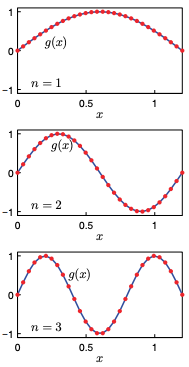
\includegraphics[width=\marginparwidth]{fig34}\captionof{figure}{The first three eigenfunctions found in 3.3. The points are the numerical eigenfunctions and the line is the exact solution.}\label{fig:17}}

	\begin{enumerate}[label=(\alph*)]
	\item  Write a program to numerically find the eigenvalues and eigenvectors
of Eq. \eqref{eq:35} using the procedure outlined above. Use $N = 30, \mu = 0.003,
T = 127,$ and $L = 1.2$. Write a loop that plots each of the eigenvectors.
You will find two infinite eigenvalues together with odd-looking eigenvectors that don\rq t satisfy the boundary conditions. These two show up
because of the two rows of the B matrix that are filled with zeros. They
are numerical artifacts with no physical meaning, so just ignore them.
The eigenvectors of the higher modes start looking jagged. These
must also be ignored because they are poor approximations to the
continuous differential equation in Eq. \eqref{eq:35}.
	\item A few of the smooth eigenfunctions are very good approximations.
Plot the eigenfunctions corresponding to $n = 1,2,3$ and compare them
with the exact solutions in Eq. \eqref{eq:38}. Since the modes include an
arbitrary scaling $g_0$, you won\rq t find the amplitudes match unless you
choose an appropriate value for $g_0$. Calculate the exact values for $\lambda$
using Eq. \eqref{eq:39} and compare them with the numerical eigenvalues.
Now compare your numerical eigenvalues for the $n = 20$ mode with
the exact solution. What is the trend in the accuracy of the eigenvalue
method?
	\item The first few values for $\lambda$ should match the resonances that you found
in 3.2(b). Go back to your calculation in 3.2(b) and make two plots
of the steady state amplitude for driving frequencies near these two
resonant values of $\lambda$. For each plot, choose a small range of frequencies that brackets the resonance frequency above and below. You
should find very large amplitudes, indicating that you are right on the
resonances.
	\end{enumerate}
	Finally let\rq s explore what happens to the eigenmode shapes when we change
the boundary conditions.

\paragraph*{P3.4}
	\marginpar{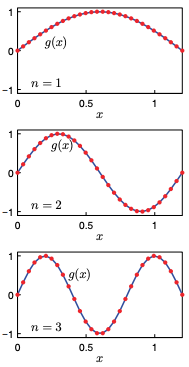
\includegraphics[width=\marginparwidth]{fig34}\captionof{figure}{The first three eigenfunctions for $3.4$ (a).}\label{fig:18}}
\begin{enumerate}[label=(\alph*)]
	\item Change your program from problem 3.3 to implement the boundary
condition  \begin{equation*}
		g^\prime(L) = 0
				\end{equation*}
				This boundary condition describes what happens if one end of the
string is free to slide up and down rather than attached to a fixed
position. Use the approximation you derived in problem 2.4(b) for the
derivative $g^\prime(L)$ to implement this boundary condition, i.e
\begin{equation*}
		g^\prime(L) \approx \frac{1}{2h}g_{N-3} - \frac{2}{h}g_{N-2} + \frac{3}{2h}g_{N-1}
				\end{equation*}Explain physically why the resonant frequencies change as they do.
				\item In some problems mixed boundary conditions are encountered, for
example\begin{equation*}
		g^\prime(L) = 2g(L)
				\end{equation*}Find the first few resonant frequencies and eigenfunctions for this
case. Look at your eigenfunctions and verify that the boundary condition is satisfied. Also notice that one of your eigenvalues corresponds
to $\omega^2$ being negative. This means that the nice smooth eigenfunction
associated with this eigenvalue is not physical in our wave resonance
problem with this boundary condition. The code snippet we gave you
above will have trouble with the np.sqrt. You can just look at the
values of $\omega^2$ instead
\end{enumerate}